\section{How does Autocorrelation work?}
Autocorrelation is matching a signal compared to a delayed version of itself. This delay between the original signal and the delay is called ‘lag'. 

``The autocorrelation \cite{Jenkins} function can be used for the following two purposes:

\begin{itemize}

    \item To detect non-randomness in data.
    
    \item To identify an appropriate time series model if the data are not random.
    
\end{itemize}

Given measurements, Y1, Y2, ..., YN at time X1, X2, ..., XN, the lag k autocorrelation function is defined as
\begin{figure}
\centering

\begin{math}
{ {r_{k} = \frac{\sum_{i=1}^{N-k}(Y_{i} - \bar{Y})(Y_{i+k} -  \bar{Y})} {\sum_{i=1}^{N}(Y_{i} - \bar{Y})^{2} }} }
\end{math}

\caption{Autocorrelation Formula}
\label{autocorrolationF}
\end{figure}

Although the time variable, X, is not used in the formula for Autocorrelation, the assumption is that the observations are equispaced.

Autocorrelation is a correlation coefficient. However, instead of a correlation between two different variables, the correlation is between two values of the same variable at times Xi and Xi+k.

In our case we use Autocorrelation to identify an appropriate time series model, hence we plot with many lags." \cite{NIST}

\subsection{How does this apply?}

The Autocorrelation coefficient has now been explained mathematically - but how can this be shown graphically? When looking at Figure \ref{ACF coefficient} and starting on the Y axis, you can see the scale goes from -1 to 1. 1 equates to a perfect match, whilst -1 is an anti-phase cycle match. 0 means there is a 0\% correlation. The X axis is the length of time of the dataset, but is not shown as a conventional measure of time (ie seconds, minutes). Instead, it is shown as rows on our dataset (as seen in the table shown in Figure \ref{data table}). If the dataset is 10,000 datapoints long, the X axis Autocorrelation coefficient graph will therefore show 10,000 as the maximum X value.  On the graph, peaks will be marked with red crosses. These are what the script looks for when identifying representative cycles.

\begin{figure}[ht]
\centering
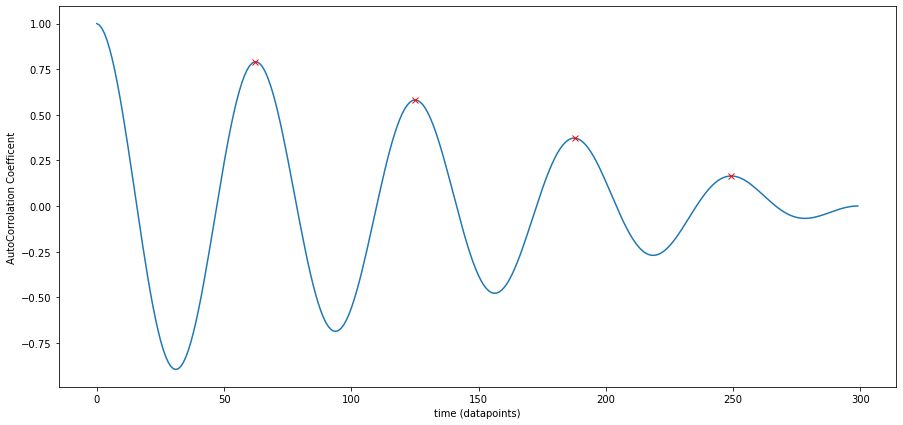
\includegraphics[scale=0.45]{images/ACF u DIAGRAM.png}
\caption{ACF tutorial}
\label{ACF coefficient}
\end{figure}

\section{Other methods of pattern recognition}
All methods and approaches of pattern recognition need to follow the approach shown in Figure \ref{fig:method}. Using the database produced by JJulien Siebert, Janek Groß, and Christof Schro \cite{DBLP:journals/corr/abs-2104-07406}, a table was made for time series data; this allows users to filter any information they need for the required task. In our case, we need to filter by pattern recognition. However, there are other classification methods available such as forecasting, classification, clustering, anomaly detection etc. Below is a list of all the libraries that fit the report's needs for pattern recognition.
\begin{figure}
    \centering

\tikzset{every picture/.style={line width=0.75pt}} %set default line width to 0.75pt        


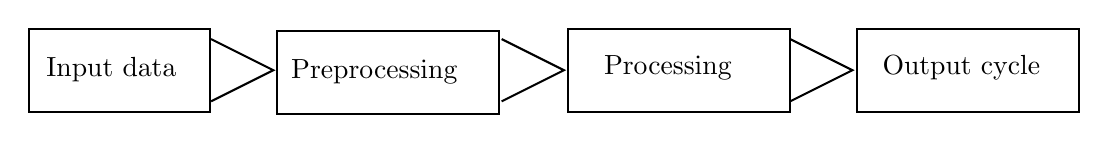
\begin{tikzpicture}[x=0.75pt,y=0.75pt,yscale=-1,xscale=1]
%uncomment if require: \path (0,300); %set diagram left start at 0, and has height of 300

%Shape: Rectangle [id:dp6164774614967738] 
\draw   (88.14,122) -- (175.44,122) -- (175.44,162) -- (88.14,162) -- cycle ;
%Shape: Rectangle [id:dp8360875880221361] 
\draw   (207.63,123) -- (314.63,123) -- (314.63,163) -- (207.63,163) -- cycle ;

%Shape: Rectangle [id:dp6039686166404709] 
\draw   (347.82,122) -- (454.82,122) -- (454.82,162) -- (347.82,162) -- cycle ;

%Shape: Rectangle [id:dp467126276166151] 
\draw   (487,122) -- (594,122) -- (594,162) -- (487,162) -- cycle ;

\draw   (176,127) -- (206,142) -- (176,157) ;
\draw   (316,127) -- (346,142) -- (316,157) ;
\draw   (455,127) -- (485,142) -- (455,157) ;

% Text Node
\draw (213.13,135.5) node [anchor=north west][inner sep=0.75pt]   [align=left] {Preprocessing};
% Text Node
\draw (363.82,133.5) node [anchor=north west][inner sep=0.75pt]   [align=left] {Processing};
% Text Node
\draw (498,133.5) node [anchor=north west][inner sep=0.75pt]   [align=left] {Output cycle};
% Text Node
\draw (95.17,134.5) node [anchor=north west][inner sep=0.75pt]   [align=left] {Input data};

\end{tikzpicture}
    \caption{}
    \label{fig:method}
\end{figure}
\subsection{Stumpy}
On 17 Jul 2019, the Stumpy library was created. This library was born from the essential research created by the  University of New Mexico, Riverside and the University of California. It ``described an exact method called STOMP for computing the matrix profile for any time series with a computational complexity of O(n2)!" \cite{law2019stumpy} 

\subsubsection{Matrix profile} 
The STUMPY library efficiently computes a matrix profile, a vector that stores the z-normalized Euclidean distance in between subsequences in a time series and its nearest neighbour. Target market is academics, data scientists, and developers. Open-sourced STUMPY, is a strong and scalable library that efficiently computes the matrixprofile according to this published study \cite{law2019stumpy}. If the reader wishes to dive deeper into the technicalities of z-normalized Euclidean distance, they can read the best paper award winner from ICDM 2017.\cite{zhu_imamura_nikovski_keogh_2017}.

\subsubsection{How can Stumpy be implemented for pattern recognition?}
Utilizing dataset A with STUMP function, the graphs in Figure \ref{Motif} were produced.
The Y axis is the z-normalized Euclidean distance shown on the bottom plot. The higher the value, the lower the ``correlation". This is illustrated by the best cycles selected, starting at the lowest points on the Matrix profile.

To automatically select the lowest point on the Matrix profile, a NumPy sorting algorithm is used to select the first point.

\begin{python}
motif_idx = np.argsort(mp[:, 0])[0]
print(f"The motif is located at index {motif_idx}")
\end{python}
The motif is located at index 85062

\begin{figure}
\centering
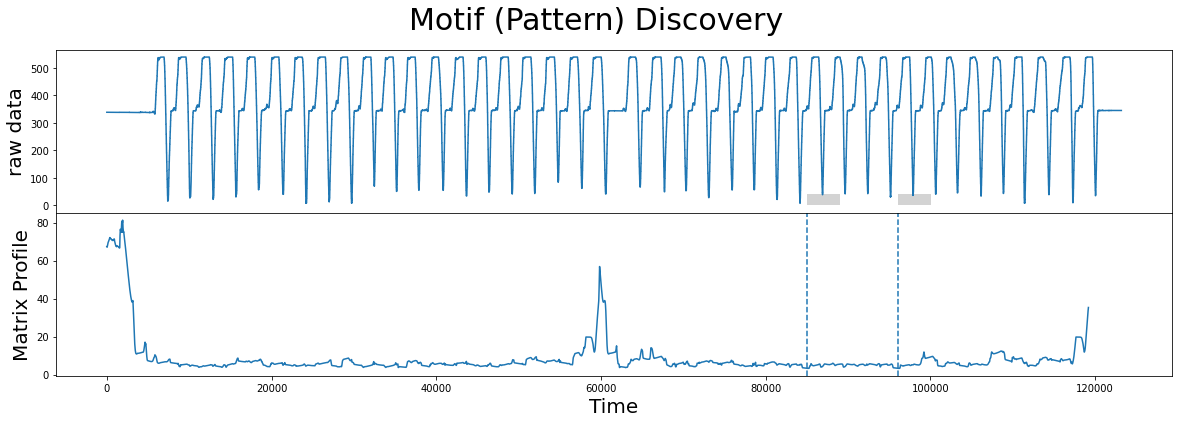
\includegraphics[scale=0.40]{images/Motif (Pattern) Discovery.png}
\caption{Motif (Pattern) Discovery}
\label{Motif}
\end{figure}
According to the documentation \cite{law2019stumpy}, to select a complete cycle the user must select the lowest point in the Matrix profile, and then add the rough length of the pattern to create the start and endpoint of the cycle.

Requiring the knowledge of the cycle length prior to running the program highlighted a major problem with stumpy. This problem means that the stumpy library cannot be used if the engineer does not know the cycle length they are after. 
\begin{python}
length = 4000
mp = stumpy.stump(datasetA['mm'], length)

\end{python}

\begin{figure}
\centering
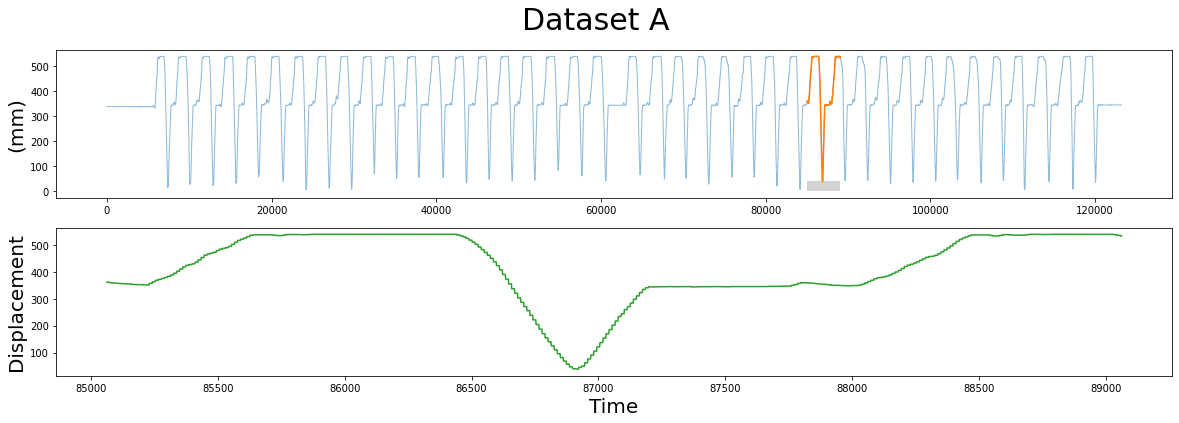
\includegraphics[scale=0.40]{images/DatasetA.png}
\caption{Motif (Pattern) Discovery}
\label{Stumpy Cycle selected}
\end{figure}

\subsection{pyts}
"pyts "is a Python library specialized in classifying time series. It seeks to make time series classification more accessible by offering pre-processing and utility tools, as well as implementations of multiple time series classification algorithms. The package includes several unit tests, and continuous integration ensures backward compatibility and code integration. The package is released under the BSD licence with three clauses.  \cite{JMLR:v21:19-763}


Unfortunately, after researching and testing the tool to see its application, it has been discovered that it does not fit the requirements. The `pyst' library uses machine learning that requires training samples before running the actual time series data, and under the methodology of the report, no training samples are provided. The function also has to find `a representative cycle' with only 1 dataset, and even though it markets itself as pattern recognition (confirmed in database paper \cite{DBLP:journals/corr/abs-2104-07406}), the`pyst' library fails to do so.

\subsection{MatrixProfile}
Here is another library based on the z-normalised Euclidean distance papers \cite{zhu_imamura_nikovski_keogh_2017}. MatrixProfile is a Python 3 library produced explicitly by the MatrixProfile Foundation for timeseries doing data mining. The MatrixProfile is a novel data structure with accompanying algorithms (regimes, stomp, motifs etc.) created by the research groups of Keogh and Mueen at UC-Riverside and the University of New Mexico. The objective of MatrixProfile is to make these algorithms accessible to both beginners and experts. This can be done by standardising basic principles and good documentation \cite{Van_Benschoten2020}. 

Unfortunately, at the time this report was taken, Python 3.10 was not supported. This stopped the author from using the CAT machine datasets for this library. However, article \cite{Van_Benschoten2020} provides Figure \ref{matrixTable} with the results of a taxi dataset conducted in New York City. These results seem promising for the report, and have an interesting automatic Discord identifier. In this context, Discord is defined as ``A time series discord indicates a subsequence with the maximum distance to its neighbor in the given time series data, which means abnormal or unusual data trends."\cite{woodbridge_wilson_rintoul_goldstein_2015}

\begin{figure}
\centering
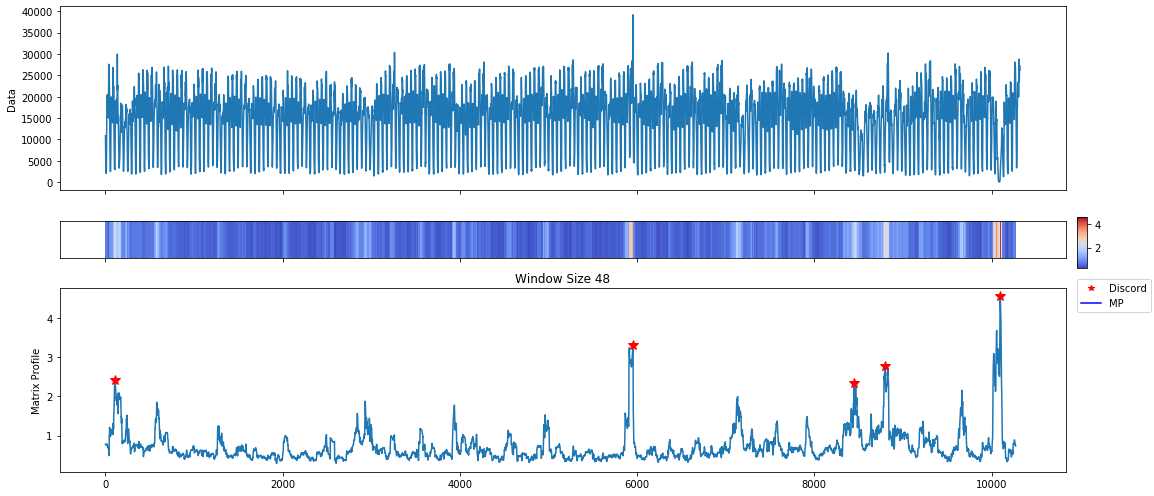
\includegraphics[scale=0.40]{images/examples_NYC_Taxis_8_2.png}
\caption{matrixTable}
\label{matrixTable}
\end{figure}

\subsection{tslearn}
``tslearn" is another library based on the Scikit-learn platform, and is a trendy Python package for machine learning. Unfortunately, this library has the same issue as MatrixProfile; it relies on training data for the AI to practice before running through the main dataset. In this case, no training data is allowed in the report's case, rendering the ``tslearn" library unsuitable.
